\chapter{Introduction}
The purpose of this project is to use generative art techniques to explore the
spaces created by the works of the artist \emph{Darrell Viner (1947-2001)}. Viner's work
included movement, sound, and light, and though primarily working with
sculpture, he produced a series of pen plotter drawings. These drawings have
been called pioneering works in the field of computer art \citep{viner_bio}.

\begin{figure}[H]
    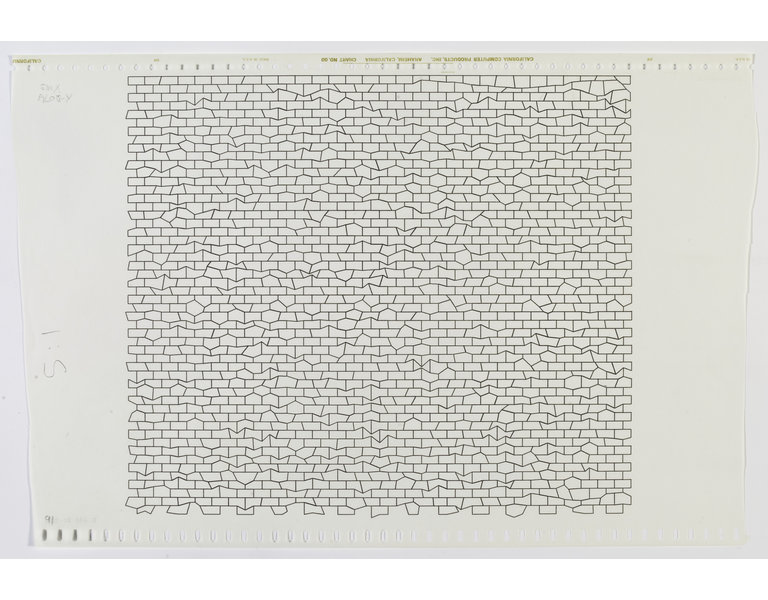
\includegraphics[scale=0.4]{viner1}
    \centering
    \caption{\emph{Darrell Viner, Untitled (1974)} \copyright Victoria and Albert Museum, London.}
\end{figure}

Generative art is any art that which is created with some system that produces
an output, it can either be art which is completed by hand (e.g. a painting)
with some system, or stochastic process. Or, more commonly art which is
generated by computer program with some initial parameters.

The project will incorporate graphics and sound to create software that can be
used to explore the landscapes present in Viner's works. The major problem that
needs to be solved in this project is creating an interface that allows the user
to interact meaningfully with the program and a set of parameters that might be
changed to produce an image.

Viner spoke about his work being like a ``townscape/landscape'': 
``Basically it is a self generating program which depends on the start
conditions. Thus by altering various aspects of the program, changes in the
final image can be achieved. Currently I am after images which have the feel and
scale of townscapes/landscapes. The program is modified depending upon whether I
consider the images to be working or not: the program has become my personal
aesthetic.'' \cite{viner_artiststatement}

These parameters may for example control the spacing of the grid, the
displacement of each point, the noise present at each vertex and so on. These
parameters should be able to be changed to create some sort of `landscape' or
`topology' that the user can explore through manipulating the program. Later on
I will detail methods for users being able to manipulate the parameters and
considerations that need to be made with respect to usability.

The program should allow for a user to generate such images and recall them
later. Ideally, the program should be more than just a show of the potential
configurations of Viner's work and itself be a unique experience for the user
and work to create a dialogue with the original work and contextualise the
user's understanding of his work.

\section{Objectives \& Deliverables}
\subsection{Objectives}

% These should be testable objectives
\begin{itemize}
    \item To create a program that allows the user to experience the works of
        Viner through the manipulation of parameters in a way that enables
        exploration and recall.
    \item Develop a catalogue of techniques to be used in generative art and
        music, and to evaluate each for relevance to the project
    \item Create an interface which allows users to navigate generated spaces
    \item Create a system such that users are able to recall a state they were
        in, and find it again
    \item As an extension of that a way of seeing all previous states, or a map
        of what the user had seen in a session
\end{itemize}

\subsection{Deliverables}
An application written for processing that should allow the user to explore a
landscape, generated to feel like Viner's work. This application should be
friendly to use and will include both graphics and sound. The feeling of some
sort of topography should be conveyed and the visual should look similar to
Viner's work. The audio will help the user navigate the space and correspond to
what is on the screen graphically in some way.

There should be another mode within the program that allows users to explore the
previous session's movements and recall what they saw. This should be easy to
understand and allow for users to see configurations of parameters they like and
save them somehow.

\section{Initial Plan}
Being that this project is exploratory in nature, an iterative approach to
development makes sense, with small prototypes being created, explored, and
built on quickly. As such I have allocated time for ideas to be developed in.

To start I will learn about processing, this library for Java makes it simple to
get a framework for graphics, of which the logical can be easily moved to some
other framework if need be. Since my tutor's previous work was written in
processing, there is already some groundwork complete to build off of. It may be
worth exploring other options like \verb|p5.js| for portability and the ability
to embed into webpages for the final implementation, \verb|p5.js| offers some
more mature sound libraries, as well as other web technologies which may be
useful for future explorations such as Geo-location and portability to mobile
devices.

\begin{center}
    \begin{ganttchart}[vgrid]{1}{12}
        \gantttitle{Week}{12}\\
        \gantttitlelist{1,...,12}{1} \\
        \ganttbar{Learning Processing}{1}{2} \\
        \ganttbar{Exploring Audio Ideas}{3}{4}
        \ganttbar{}{7}{9} \\
        \ganttbar{Exploring Polygon Drawing}{5}{9} \\
        \ganttbar{Creating Proof of Concept demo with grid and audio}{6}{7} \\
        \ganttbar{Final Proof of Concept before end of year}{9}{12} \\
        \ganttbar{Writing Report}{1}{12}
    \end{ganttchart}
\end{center}

\section{Risk Mitigation}
Since this project is fairly isolated in nature, there aren't a lot of risks to
consider.

If the project had relied on access to the art directly, the COVID-19 pandemic
would have affected it, but we mitigated this risk by setting the scope of the
project to not include access to the art.

Another risk in this project is scope-creep; since the project is artistic it
can be very easy to have many ideas whilst losing the original focus. To combat
this I will set specific objectives and deliverables and reach those before
exploring any further options.
